%% 
%% Copyright 2007-2019 Elsevier Ltd
%% 
%% This file is part of the 'Elsarticle Bundle'.
%% ---------------------------------------------
%% 
%% It may be distributed under the conditions of the LaTeX Project Public
%% License, either version 1.2 of this license or (at your option) any
%% later version.  The latest version of this license is in
%%    http://www.latex-project.org/lppl.txt
%% and version 1.2 or later is part of all distributions of LaTeX
%% version 1999/12/01 or later.
%% 
%% The list of all files belonging to the 'Elsarticle Bundle' is
%% given in the file `manifest.txt'.
%% 
%% Template article for Elsevier's document class `elsarticle'
%% with harvard style bibliographic references

%%\documentclass[preprint,12pt,authoryear]{elsarticle}

%% Use the option review to obtain double line spacing
 \documentclass[authoryear,preprint,review,12pt]{elsarticle}

%% Use the options 1p,twocolumn; 3p; 3p,twocolumn; 5p; or 5p,twocolumn
%% for a journal layout:
%% \documentclass[final,1p,times,authoryear]{elsarticle}
%% \documentclass[final,1p,times,twocolumn,authoryear]{elsarticle}
%% \documentclass[final,3p,times,authoryear]{elsarticle}
%% \documentclass[final,3p,times,twocolumn,authoryear]{elsarticle}
%% \documentclass[final,5p,times,authoryear]{elsarticle}
%% \documentclass[final,5p,times,twocolumn,authoryear]{elsarticle}

%% For including figures, graphicx.sty has been loaded in
%% elsarticle.cls. If you prefer to use the old commands
%% please give \usepackage{epsfig}

%% The amssymb package provides various useful mathematical symbols
 \usepackage{amssymb}
 \usepackage{amsmath}
%% The amsthm package provides extended theorem environments
%% \usepackage{amsthm}

%% The lineno packages adds line numbers. Start line numbering with
%% \begin{linenumbers}, end it with \end{linenumbers}. Or switch it on
%% for the whole article with \linenumbers.
%% \usepackage{lineno}

\journal{Earth and Planetary Science Letters}

\newcommand\Gr{\mbox{\textit{Gr}}} %Grashof number

\begin{document}

\begin{frontmatter}

%% Title, authors and addresses

%% use the tnoteref command within \title for footnotes;
%% use the tnotetext command for theassociated footnote;
%% use the fnref command within \author or \address for footnotes;
%% use the fntext command for theassociated footnote;
%% use the corref command within \author for corresponding author footnotes;
%% use the cortext command for theassociated footnote;
%% use the ead command for the email address,
%% and the form \ead[url] for the home page:
%% \title{Title\tnoteref{label1}}
%% \tnotetext[label1]{}
%% \author{Name\corref{cor1}\fnref{label2}}
%% \ead{email address}
%% \ead[url]{home page}
%% \fntext[label2]{}
\cortext[cor1]{Corresponding author: paul.jarvis@unige.ch}
%% \address{Address\fnref{label3}}
%% \fntext[label3]{}

\title{Collective sedimentation from ash-clouds: insights from experimental buoyant, particle-laden gravity currents}

%% use optional labels to link authors explicitly to addresses:
%% \author[label1,label2]{}
%% \address[label1]{}
%% \address[label2]{}

\author[label1]{Paul A. Jarvis\corref{cor1}}
\author[label1]{Allan Fries}
\author[label1]{Jonathan Lemus}
\author[label1]{Costanza Bonadonna}
\author[label2]{Amanda Clarke}
\author[label3]{Irene Manzella}
\author[label4]{Jeremy Phillips}

\address[label1]{Department of Earth Sciences, University of Geneva, Rue des Mar{\"i}chers, Geneva, 1205, Switzerland}
\address[label2]{School of Earth and Space Exploration, Arizona State University, ISTB4-BLDG75, 781 E Terrance Mall, Tempe, AZ, 85287-6004, USA}
\address[label3]{School of Geography, Earth and Envrionmental Sciences, Univeristy of Plymouth, Drake Circus, Plymouth, PL4 8AA, UK}
\address[label4]{School of Earth Sciences, University of Bristol, Wills Memorial Building, Queens Road, Bristol, BS8 1RJ, UK}

\begin{abstract}
%% Text of abstract

\end{abstract}

%%Graphical abstract
\begin{graphicalabstract}
%\includegraphics{grabs}
\end{graphicalabstract}

%%Research highlights
\begin{highlights}
\item Research highlight 1
\item Research highlight 2
\end{highlights}

\begin{keyword}
%% keywords here, in the form: keyword \sep keyword

%% PACS codes here, in the form: \PACS code \sep code

%% MSC codes here, in the form: \MSC code \sep code
%% or \MSC[2008] code \sep code (2000 is the default)

\end{keyword}

\end{frontmatter}

%% \linenumbers

%% main text
\section{Introduction}
\label{sec:intro}

The volcanic ash produced by explosive volcanic eruptions is an economic and societal hazard. Fine ash which is breathed in can cause respiratory health problems in humans and animals \citep{Kampa07, Anderson12, WHO13, Baxter15}. Agriculturally, ash deposits can contaminate human and livestock food and water supplies, as well as cover crops \citep{Cook81, Cronin98, Wilson11, Craig16}. More generally, ash can cause buildings to collapse and damage electrical power systems \citep{Wilson14, Craig16}. A well-publicised impact is that on the aviation industry, whereby the risk of damage to airplane engines can lead to costly shutdowns of airspace \citep{Budd11, Elissondo16}. The mechanisms of ash dispersal and sedimentation therefore need to be understood in order for accurate hazard and risk assessments to be carried out.

Key tools used for hazard assessment are ash dispersal models which aim to simulate the transport of volcanic ash in the atmosphere \citep{Witham07, Bonadonna12, Folch12}. These have been used to produce operational forecasts of ash clouds \citep{Scollo09, Webster12} or to produce hazard maps which can be used in decision making \citep{Bonadonna05, Macedonio05, Folch10}. These models rely on accurate parameterisations of ash sedimentation processes. However, it is often assumed that ash settles at its terminal fall velocity \citep{Hazen04}, as determined from its size and the density contrast with the surrounding atmosphere \citep{Clift71, Ganser93}. Such a scheme predicts that the model grain size of deposited ash should decrease monotonically with distance from the vent \citep{Bursik92, Sparks92}. Deposits, however, sometimes record more complicated features such as bimodal size distributions whilst remotely sensed GSDs of the ash plume from the 2010 eruption of Eyjafjallaj{\"o}kull also showed that the effective ash radius did not monotonically decrease with distance from the vent \citep{Bonadonna11}. Indeed, it is increasingly apparent that collective sedimentation processes can strongly control the sedimentation of ash. One commonly cited mechanism is ash aggregation, whereby ash particles stick together, increasing their effective size and thus their fall velocity \citep{Carey82, Sorem82, Lane93, Bonadonna11, Brown12}. Another possibility though is that collective sedimentation can occur through the occurence of convective instabilties which drive larger scale fluid motions that can drive ash sedimentation through downward-propagating finger structures \citep{Bonadonna02, Bonadonna11, Carrazo12, Manzella15, Scollo17}. These arise due to the formation of a gravitationally unstable interfacial layer at the base of ash clouds, which has previously been called the particle boundary layer or PBL \citep{Carrazo12}.

Despite recent progress in understanding how convective instabilties form and evolve, there remains a number of key unanswered questions. In particular, no consideration has been given to the role of background velocity shear, which will be present due to buoyant spreading of the cloud and/or wind drag \citep{Johnson15}. In this study, we explore how the presence of shear at the base of volcanic clouds, due to buoyant spreading, can influence collective settling behaviour. In particular, we show that there is a regime where Kelvin-Helmholtz shear instabilties \citep{Helmholtz68, Kelvin71} can interact with settling-driven gravitational instabilities \citep{Hoyal99, Blanchette05} to produce larger fingers that can enhance the sedimentation of fine ash.

\subsection{Settling-driven gravitational instabilities}
\label{subsec:SDGI}

Settling-driven gravitational instabilities (SDGIs) can occur when a particle suspension is emplaced above a denser fluid \citep{Hoyal99, Blanchette05}. Although this initial configuration is stable (Figure~\ref{fig:dens_prof}a), as particles settle into the lower layer, they can form an interfacial layer which is denser than the underlying fluid (Figure~\ref{fig:dens_prof}b). This unstable layer has previously been called the particle boundary layer (PBL) \citep{Carrazo12}. Once this PBL reaches a critical thickness, it can destabilise and generate downward-propagating fingers \citep{Hoyal99}. SDGIs are similar to double-diffusive instabilities, where instead of particle-settling, the motion of the density-controlling components is governed by diffusion \citep{Stern60}. For the purposes of this study, we are intrested in cases where the settling velocity of the particles $V_{\text{s}}$ is sufficiently high that diffusion can be neglected and double-diffusive instabilties do not occur.

\begin{figure}[ht!]
  \centerline{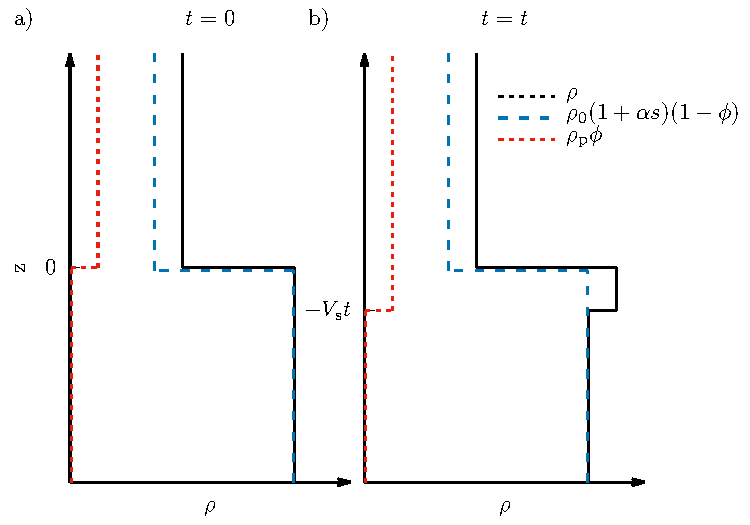
\includegraphics[width=0.9\textwidth]{dens_prof.pdf}}
  \caption{Sketch after \citet{Burns12} showing the formation mechanism of settling-driven gravitational instabilities. a) The initial configuration. The upper layer ($z > 0$) is a particle suspension of volume fraction $\phi$ in a fluid of density $\rho_{0}$. The lower layer ($z < 0$) is a single-phase fluid but includes a density altering component (dissolved substance or temperature). Thus the density of the lower layer is given by $\rho_{0}(1 + \alpha s)$ where $\alpha$ is the expansivity and $s$ is the component concentration (or temperature). Throughout the tank, the blue and red lines represent the contributions of the fluid and particle phases, respectively, to the bulk density, which is given by the black line. b) The configuration after some time $t$. The front of the suspension has desceded a distance $V_{\text{s}} t$ where $V_{\text{s}}$ is the settling velocity of individual particles. This has generated an interfacial region with an unstable density configuration.}
  \label{fig:dens_prof}
\end{figure}

SDGIs are important in geological settings as the downward velocity of the generated fingers are greater than the settling velocities of individual particles. This creates the potential for enhancing the sedimentation rate from buoyant particle suspensions. Such a hypothesis was first put forward by \citet{Bradley65} to explain rapid sedimentation of sediment in eutrophic lakes \citep{Nipkow20}. In recent years, the study of SDGIs has focussed on two applications: sedimentation from volcanic clouds \citep{Carrazo12, Manzella15, Scollo17}; and sedimentation from hypopycnal currents \citep{Chen97, Parsons01, Snyder11, Rouhnia15, Rouhnia17, Jazi16, Jazi19}.

To allow a more quantitative description of SDGIs that can be applied to multiple applications, we let the fluid have a base density of $\rho_{0}$. We then allow that the density of the fluid can be altered by a single component, such as a solute or temperature. Assuming only small changes to density, the fluid density can be parameterised as $\rho_{f}(\mathbf{x}, t) = \rho_{0} [1 + \alpha s(\mathbf{x}, t)]$ where $s$ is the concentration of the solute or the temperature, and $\alpha$ is the corresponding expansivity. Furthermore, $s$ is considered to be a function of space $\mathbf{x}$ and time $t$. Meanwhile, the particle conentration is represented by $\phi(\mathbf{x}, t)$ and the density of the particle phase is $\rho_{\text{p}}$. Thus, the bulk density at any $\mathbf{x}$ and $t$ is given by

\begin{equation}
  \label{equ:bulk_dens}
  \rho(\mathbf{x}, t) = \rho_{\text{p}} \phi(\mathbf{x}, t) + \rho_{0} [1 + \alpha s(\mathbf{x}, t)] [1 - \phi(\mathbf{x}, t)].
\end{equation}

Considering the idealised situation presented in Figure~\ref{fig:dens_prof}, if the initial particle volume fraction of the upper layer is $\phi_{0}$ and the initial solute concentration of the lower layer is $s_{0}$, then, from equation~\ref{equ:bulk_dens}, the densities of upper and lower layers, and the unstable PBL can be expressed as

\begin{equation}
  \label{equ:up_dens}
  \rho_{\text{u}} = \rho_{\text{p}} \phi_{0} + \rho_{0} (1 - \phi_{0}),
\end{equation}

\begin{equation}
  \label{equ:low_dens}
  \rho_{\text{l}} = \rho_{0} (1 + \alpha s_{0}),
\end{equation}

and

\begin{equation}
  \label{equ:PBL_dens}
  \rho_{\text{PBL}} = \rho_{\text{p}} \phi_{0} + \rho_{0} (1 + \alpha s_{0}) (1 - \phi_{0}),
\end{equation}

respectively. Since it is the interface between the PBl and the lower-layer that is unstable, the relevant choice of reduced gravity for the study of SDGIs is \citep{Davies_Wykes14}

\begin{equation}
  \label{equ:red_grav_PBL}
  g^{\prime}_{\text{PBL}} = \frac{2 (\rho_{\text{PBL}} - \rho_{\text{l}}) g}{(\rho_{\text{PBL}} + \rho_{\text{l}})} = 2 A g,
\end{equation}

where $A = (\rho_{\text{PBL}} - \rho_{\text{l}}) / (\rho_{\text{PBL}} + \rho_{\text{l}})$ is the Atwood number \citep{Sharp84}.

\citet{Hoyal99} developed two criteria for settling-driven instabilities to develop. The first arises from an analogy with thermal convection; defining $\delta$ to be the PBL thickness, a Grashof number $\Gr = \frac{g^{\prime}_{\text{PBL}} \delta^{3}}{\nu^{2}}$ \citep{Turner79}, where $\nu$ is the kinematic viscosity of the fluid, can be defined as the ratio of buoyancy forces which act to destabilise the PBL and viscous forces which resist this overturning. Therefore, $\Gr$ must exceed a critical value $\Gr_{\text{c}}$, corresponding to a critical PBL thickness $\delta = \delta_{\text{c}}$, at which the PBL can detatch and form fingers. By analogy with thermal convection, \citet{Hoyal99} estimated that $\Gr_{\text{c}} = 10^{3}$. The second criteria is that the individual settling velocity of the particles $V_{\text{s}}$ must be less than the downward velocity of the generated fingers $V_{\text{f}}$; otherwise particles will settle individually. 

\subsection{Stratified shear}
\label{subsec:strat_shear}

Whilst many of the experimental and numerical studies of SDGIs have considered static configurations \citep{Chen97, Hoyal99, Blanchette05, Yu14, Burns15, Manzella15, Rouhnia15, Jazi16, Scollo17}, both volcanic clouds and hypopycnal currents are examples of stratified shear flows, where there is a velocity gradient across a density interface. In fact, the effect of shear on SDGIs has not received extenive consideration. Some experimental studies have considered particle sedimentation from surface propagating gravity currents \citep{Maxworthy99, Parsons01, McCool04, Sutherland18, Jazi19} whilst there has also been some theoretical treatment \citep{Farenzena17, Konopliv18}. One question that remains to be addressed is for what conditions does shear enhance or inhibit sedimentation? It also remains to be understood how SDGIs can interact with shear instabilities. In stratified shear flows, three canonical instabilities can arise \citep{Eaves19}: Kelvin-Helmholtz (KH) \citep{Helmholtz68, Kelvin71}, Holmboe \citep{Holmboe62} and Taylor-Caulfied (TC) \citep{Taylor31, Caulfield95}. Of particular interest would be a predictive description of the flow behaviour for different conditions and a parameterisation for the sedimentation rate.

\subsection{Gravity currents}
\label{subsec:grav_curr}

In this study, we generate shear between two density-stratified layers by allowing the upper layer to propagate as a buoyant gravity current, where the horizontal motion is generated by the difference in hydrostatic pressure in the two fluids. For an ideal, energy-conserving current, where mixing between the current and the ambient is negligible, the Froude number of the current is predicted to be \citep{Benjamin68}

\begin{equation}
  \label{equ:Froude}
  Fr = \frac{U}{(g^{\prime} H)^{1/2}} = \frac{1}{2},
\end{equation}

where $U$ is the spreading velocity of the current, $g^{\prime} = (\rho_{\text{l}} - \rho_{\text{u}}) g/ \rho_{\text{l}}$ is the reduced gravity of the current, $H$ is the depth of the total fluid volume and $\rho_{\text{u}}$ is the density of the lower, ambient fluid.
\section{Methods}
\label{sec:method}

Experiments were performed in a perspex flume of internal length 353 cm, width (12.2 $\pm$ 0.5) cm and depth 50 cm (Figure~\ref{fig:setup}). The uncertainty on the width is due to bowing of the tank walls. During the experimental setup, two removable gates can be placed at 24 and 53 cm, respectively, from the left-hand end, creating three sections. The left-most section takes no part in the experiment, whilst the short middle section is where the particle suspension is prepared, and is referred to as the gated section (length 27 cm). The remaining length of the flume is called the environment (length 3m).

\begin{figure}[ht!]
  \centerline{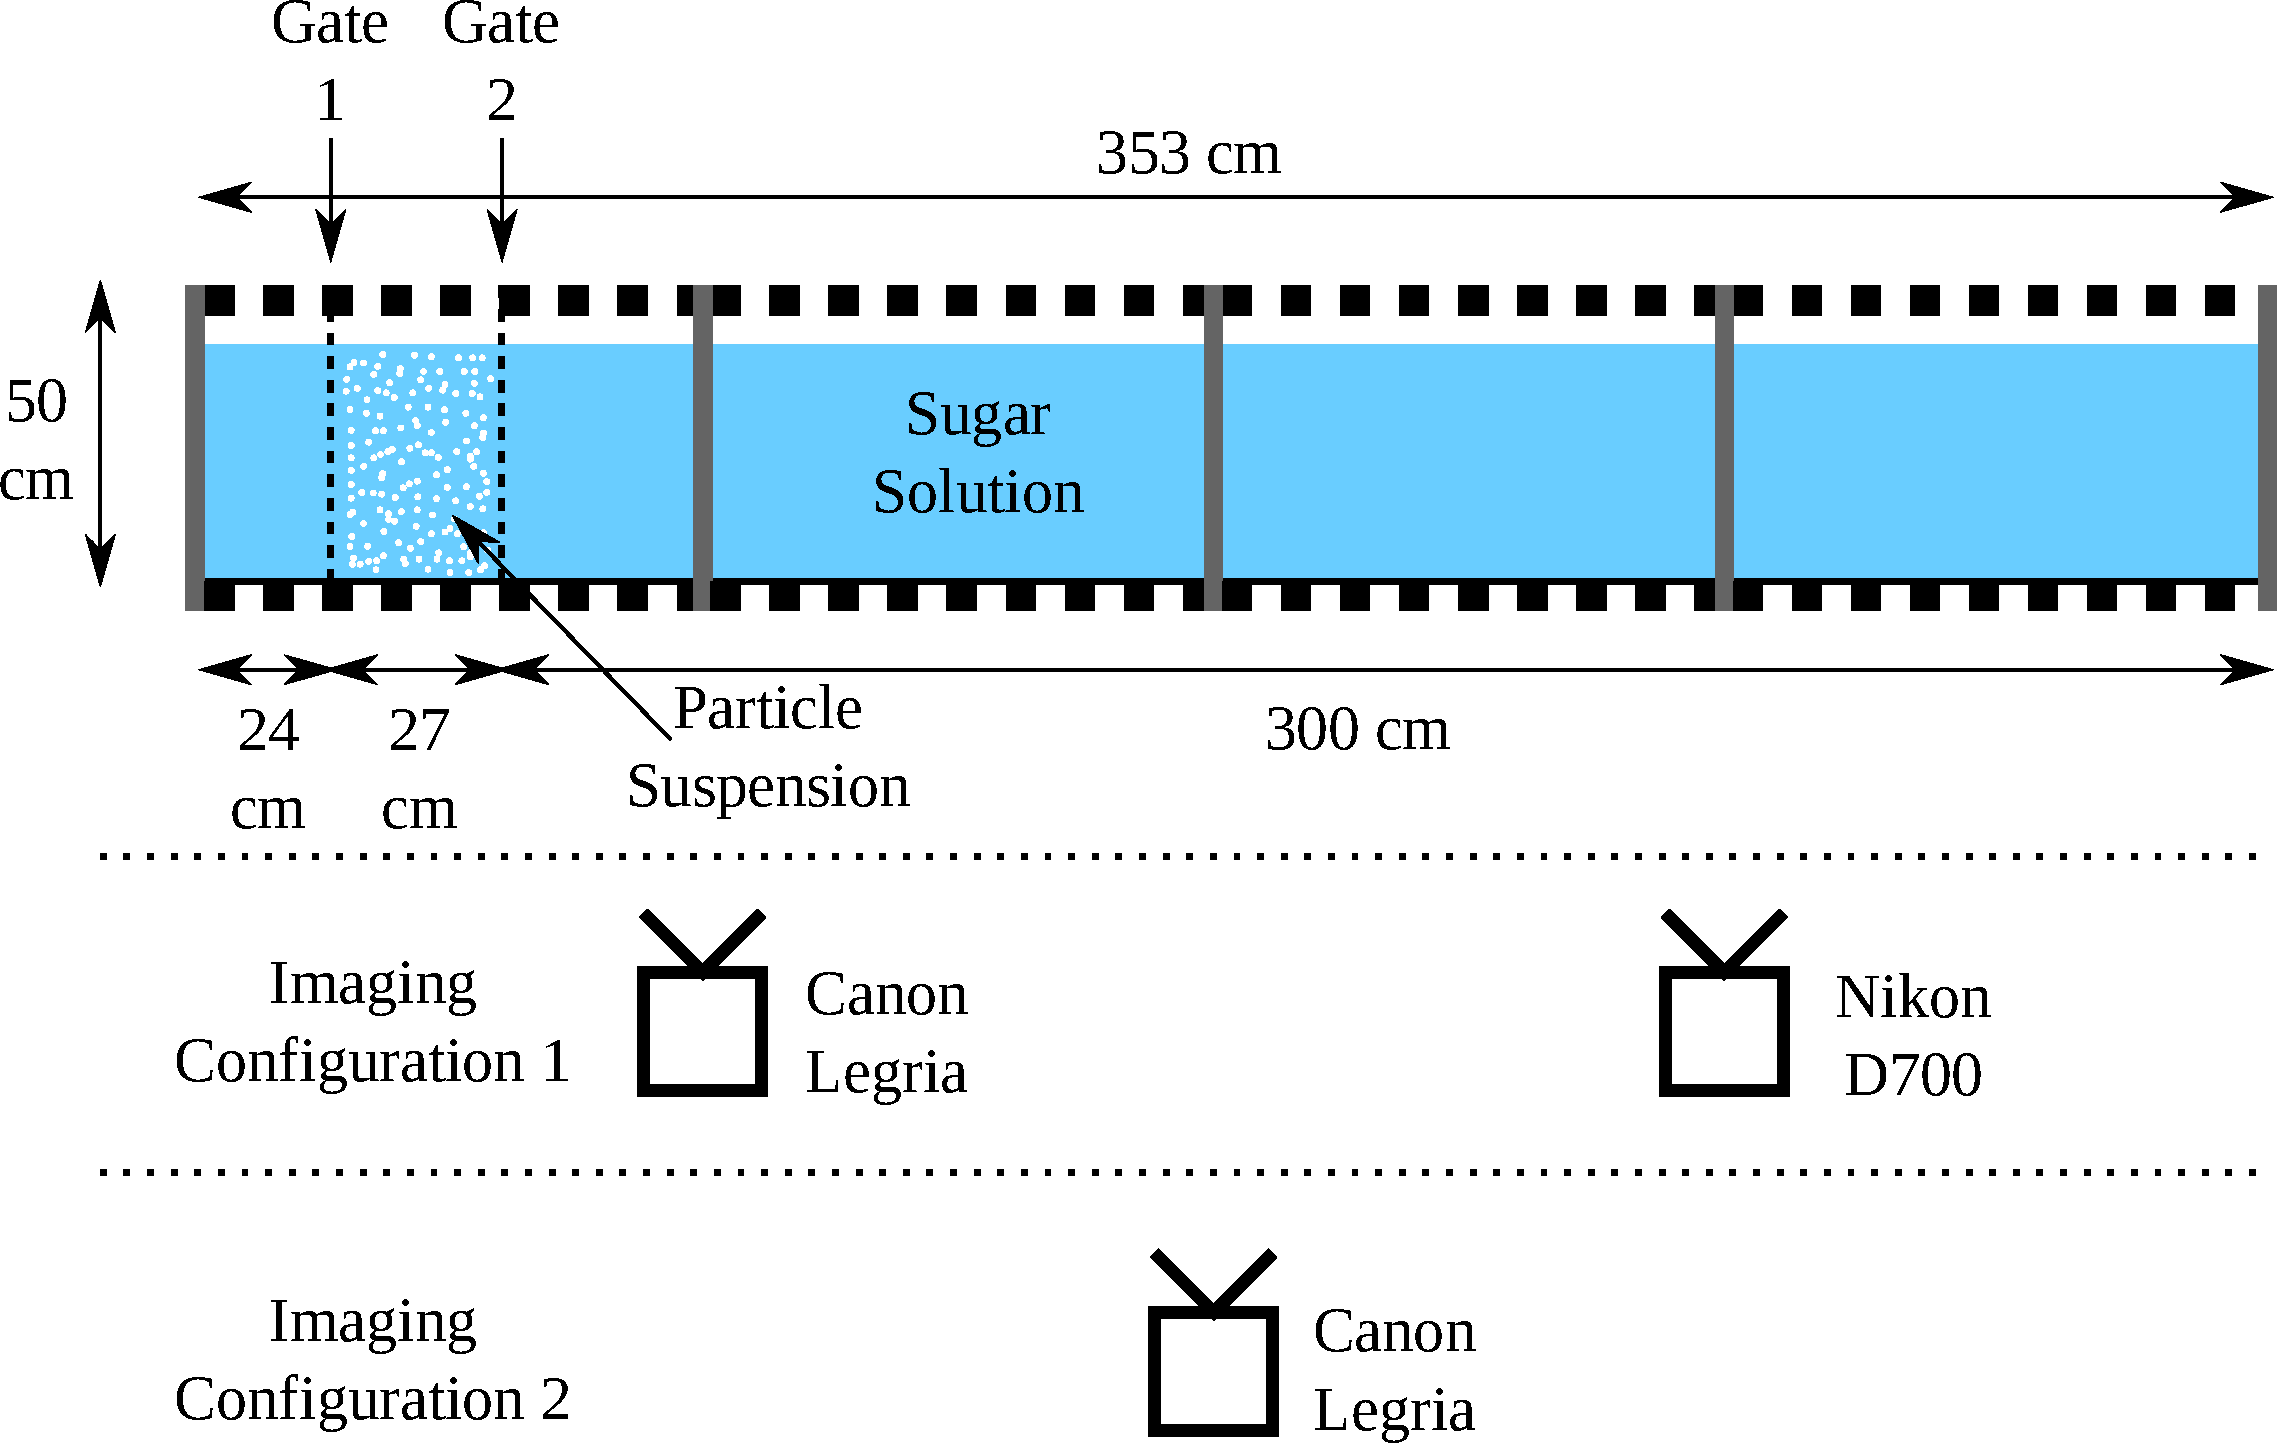
\includegraphics[width=0.9\textwidth]{setup.pdf}}
  \caption{Sketch showing the experimental setup. The flume is separated into three section separated by two gates. The leftmost section is not involved in the experiment. The rightmost section is a sugar solution of constant density whereas the section between gates 1 and 2 is a mixture of fresh water and ballotini. The concentration of particles is varied between experiments. The experiment is initiated by removing gate 2. Experiments were imaged using one of two configurations. }
  \label{fig:setup}
\end{figure}

The flume sits within a metal framework. Three vertical supports, each 3cm thick, at distances of 87 cm, 173.5 cm and 260 cm from the left-hand end prevent bowing. This effectively separates the flume into four, nearly equal, section. Behind each section a backing board is placed. For experiments with no particles, red or blue food colouring is added to the current and the backing board is white. Otherwise the boards are black. The top 5 cm of each board is a row of (5 $\times$ 5) cm$^{2}$ squares, alternating in colour from black-to-white. Meanwhile, at the base of the tank, tape is used to create a similar scale.

The day before an experiment, the flume is filled up to a depth of 47.5 cm. Separately, the desired mass of sugar is completely disolved in approximately 15 l of water. The flume and sugar solution are then both allowed to equilibrate to room temperature overnight. The next day, the flume is imaged (single frame) in its current configuration. In some experiments, the whole flume was imaged using a Canon Legria HFG40. In others, this camera was position closer to the tank, but only imaged the left-hand half of the flume, whilst the right-hand half was imaged using a Nikon D700 (DSLR). The captured frame(s) are used as reference images using the top(back) and bottom(front) scales. By capturing the image with the back scale partially submerged, it is possible to correct position measurements for distortion due to the refractive index (RI) of the water.

The flume water level is then lowered until it is of a depth of approximately 36.5 cm. Gates 1 and 2 are then put in place. The sugar solution is then added to the envrionment section. The gated section is then topped up with water until the water depth there is the same as the environment. This procedure results in a water depth of approximately 40 cm. The environment section is rigorously stirred. The RI of fluid from four positions in the environment section (top and bottom, near and far from the gate) is measured using a refractometer to ensure a uniform density. The RI of the gated section is also measured to check that there has been no significant leakage of sugar solution through the gate. A calibrated digital thermometer is used to measure the temperature of both sections. In all experiments, the maximum difference in temperature between the sections was 0.1 $^{\circ}$C.

Recording of the experiment then begins. The required mass of particles is added to the gated section which is thoroughly stirred to ensure a uniform particle concentration. Finally, gate 2 is removed and the particle suspension spreads along the free surface as a buoyant gravity current. Once the current head reaches the end of the tank, gate 2 is returned to its position and recording stops. 

The particles used were glass spheres with a density of (2.519 $\pm$ ??) g cm$^{-3}$, as measured by helium pycnometry using an Ultrapyc 1200e. They had a unimodal size distribution centred on a mode of 36 $\mu$m and a standard deviation of 12 $\mu$m, as determined from static light scattering using a Bettersizer S3 Plus. Figure~\ref{fig:size_dist} shows the measured size distribution of the particles. 

\begin{figure}[ht!]
  \centerline{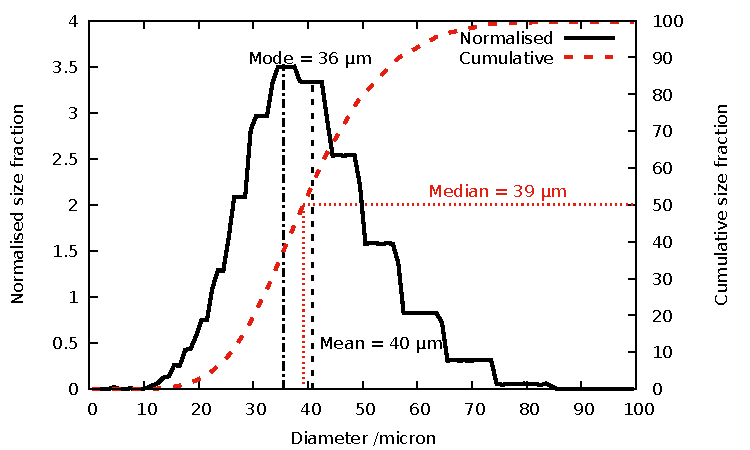
\includegraphics[width=0.9\textwidth]{unsieved_dist.pdf}}
  \caption{Normalised and cumulative volume-weighted size distributions of the particles used in the experiments.}
  \label{fig:size_dist}
\end{figure}

\section{Results}
\label{sec:res}

\subsection{Currents without particles}
\label{subsec:res_no_parts}

Figure~\ref{fig:GC3} shows the evolution of the current in experiment GC3.

\begin{figure}[ht!]
  \centerline{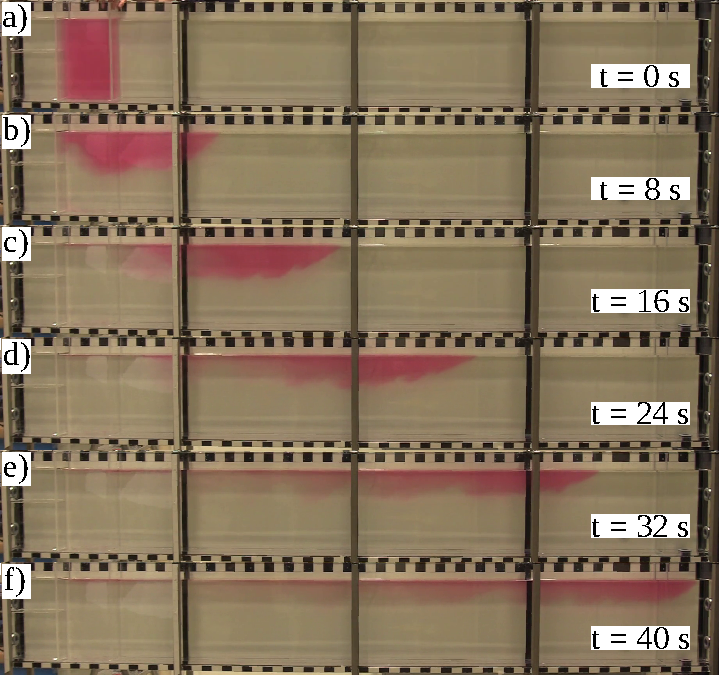
\includegraphics[width=0.9\textwidth]{GC3.pdf}}
  \caption{Sequence of images showing experiment GC3 ($\phi$ = 0, $g\prime$ = 0.162 m s$^{-2}$). }
  \label{fig:GC3}
\end{figure}

Figure~\ref{fig:GC9} shows the evolution of the current in experiment GC9.

\begin{figure}[ht!]
  \centerline{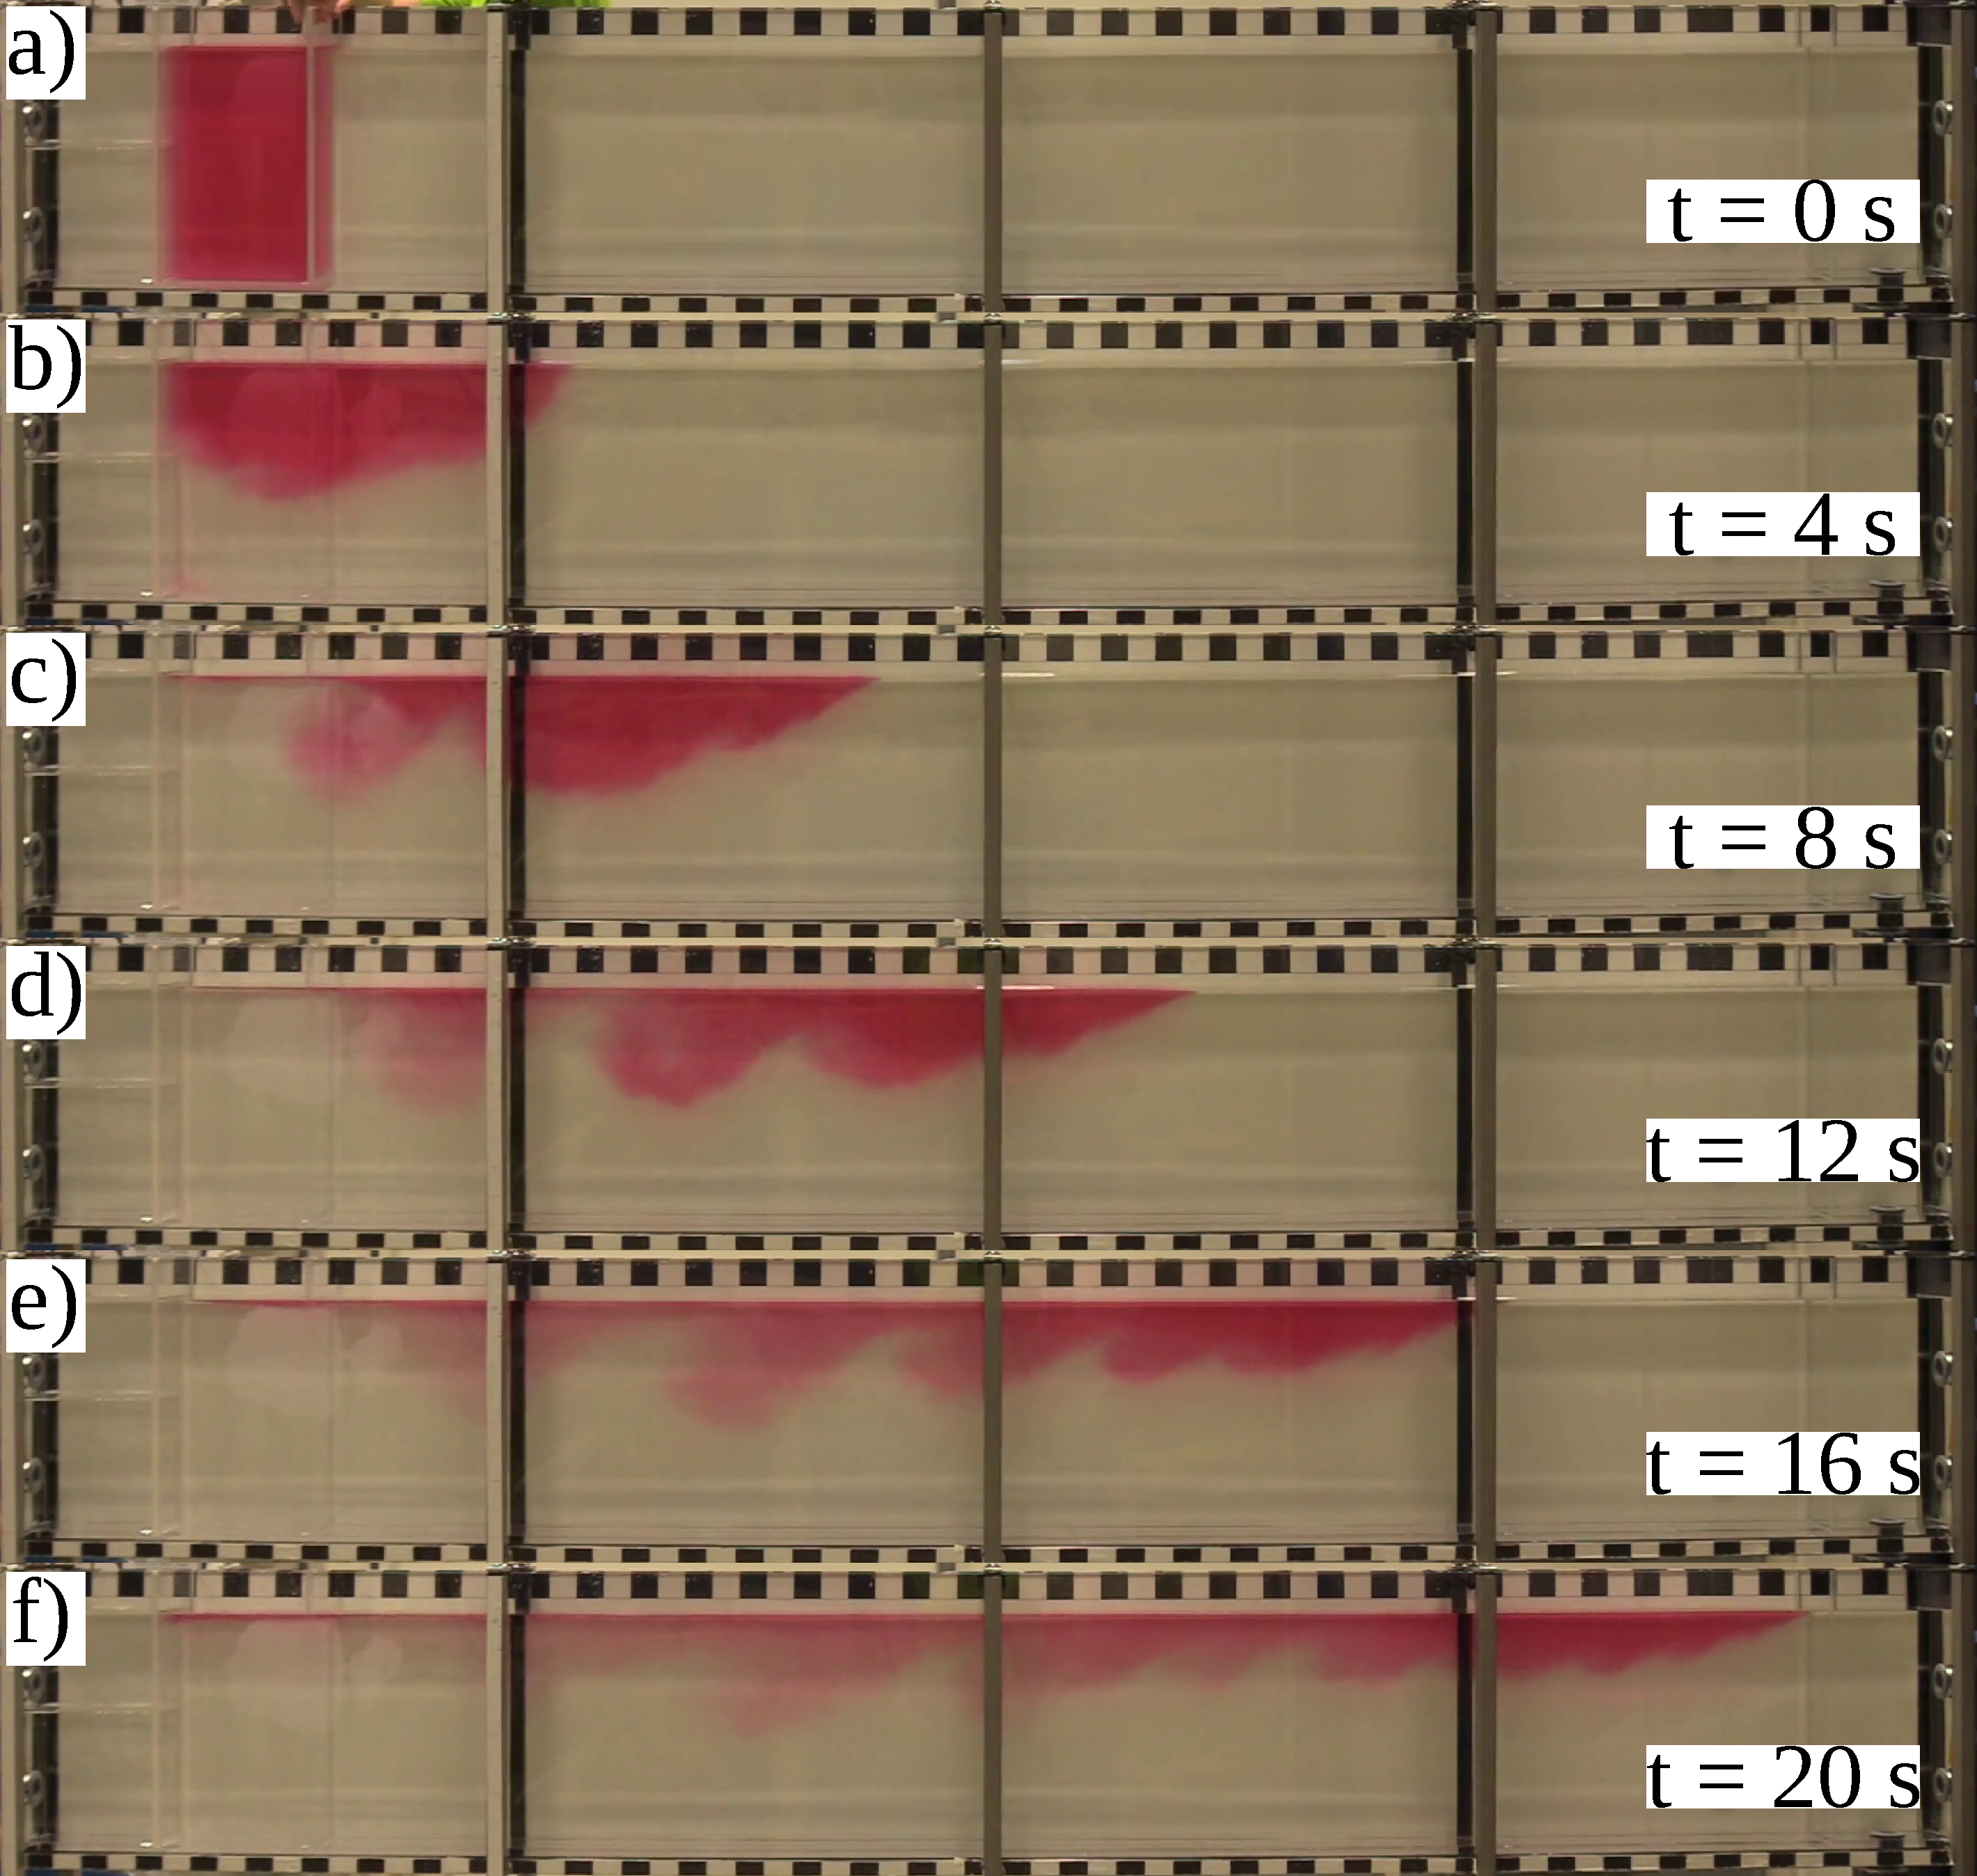
\includegraphics[width=0.9\textwidth]{GC9.pdf}}
  \caption{Sequence of images showing experiment GC9 ($\phi$ = 0, $g\prime$ = 0.563 m s$^{-2}$). }
  \label{fig:GC9}
\end{figure}

\subsection{Particle-bearing currents}
\label{subsec:res_w_parts}

Figure~\ref{fig:GC42} shows the evolution of the current in experiment GC42.

\begin{figure}[ht!]
  \centerline{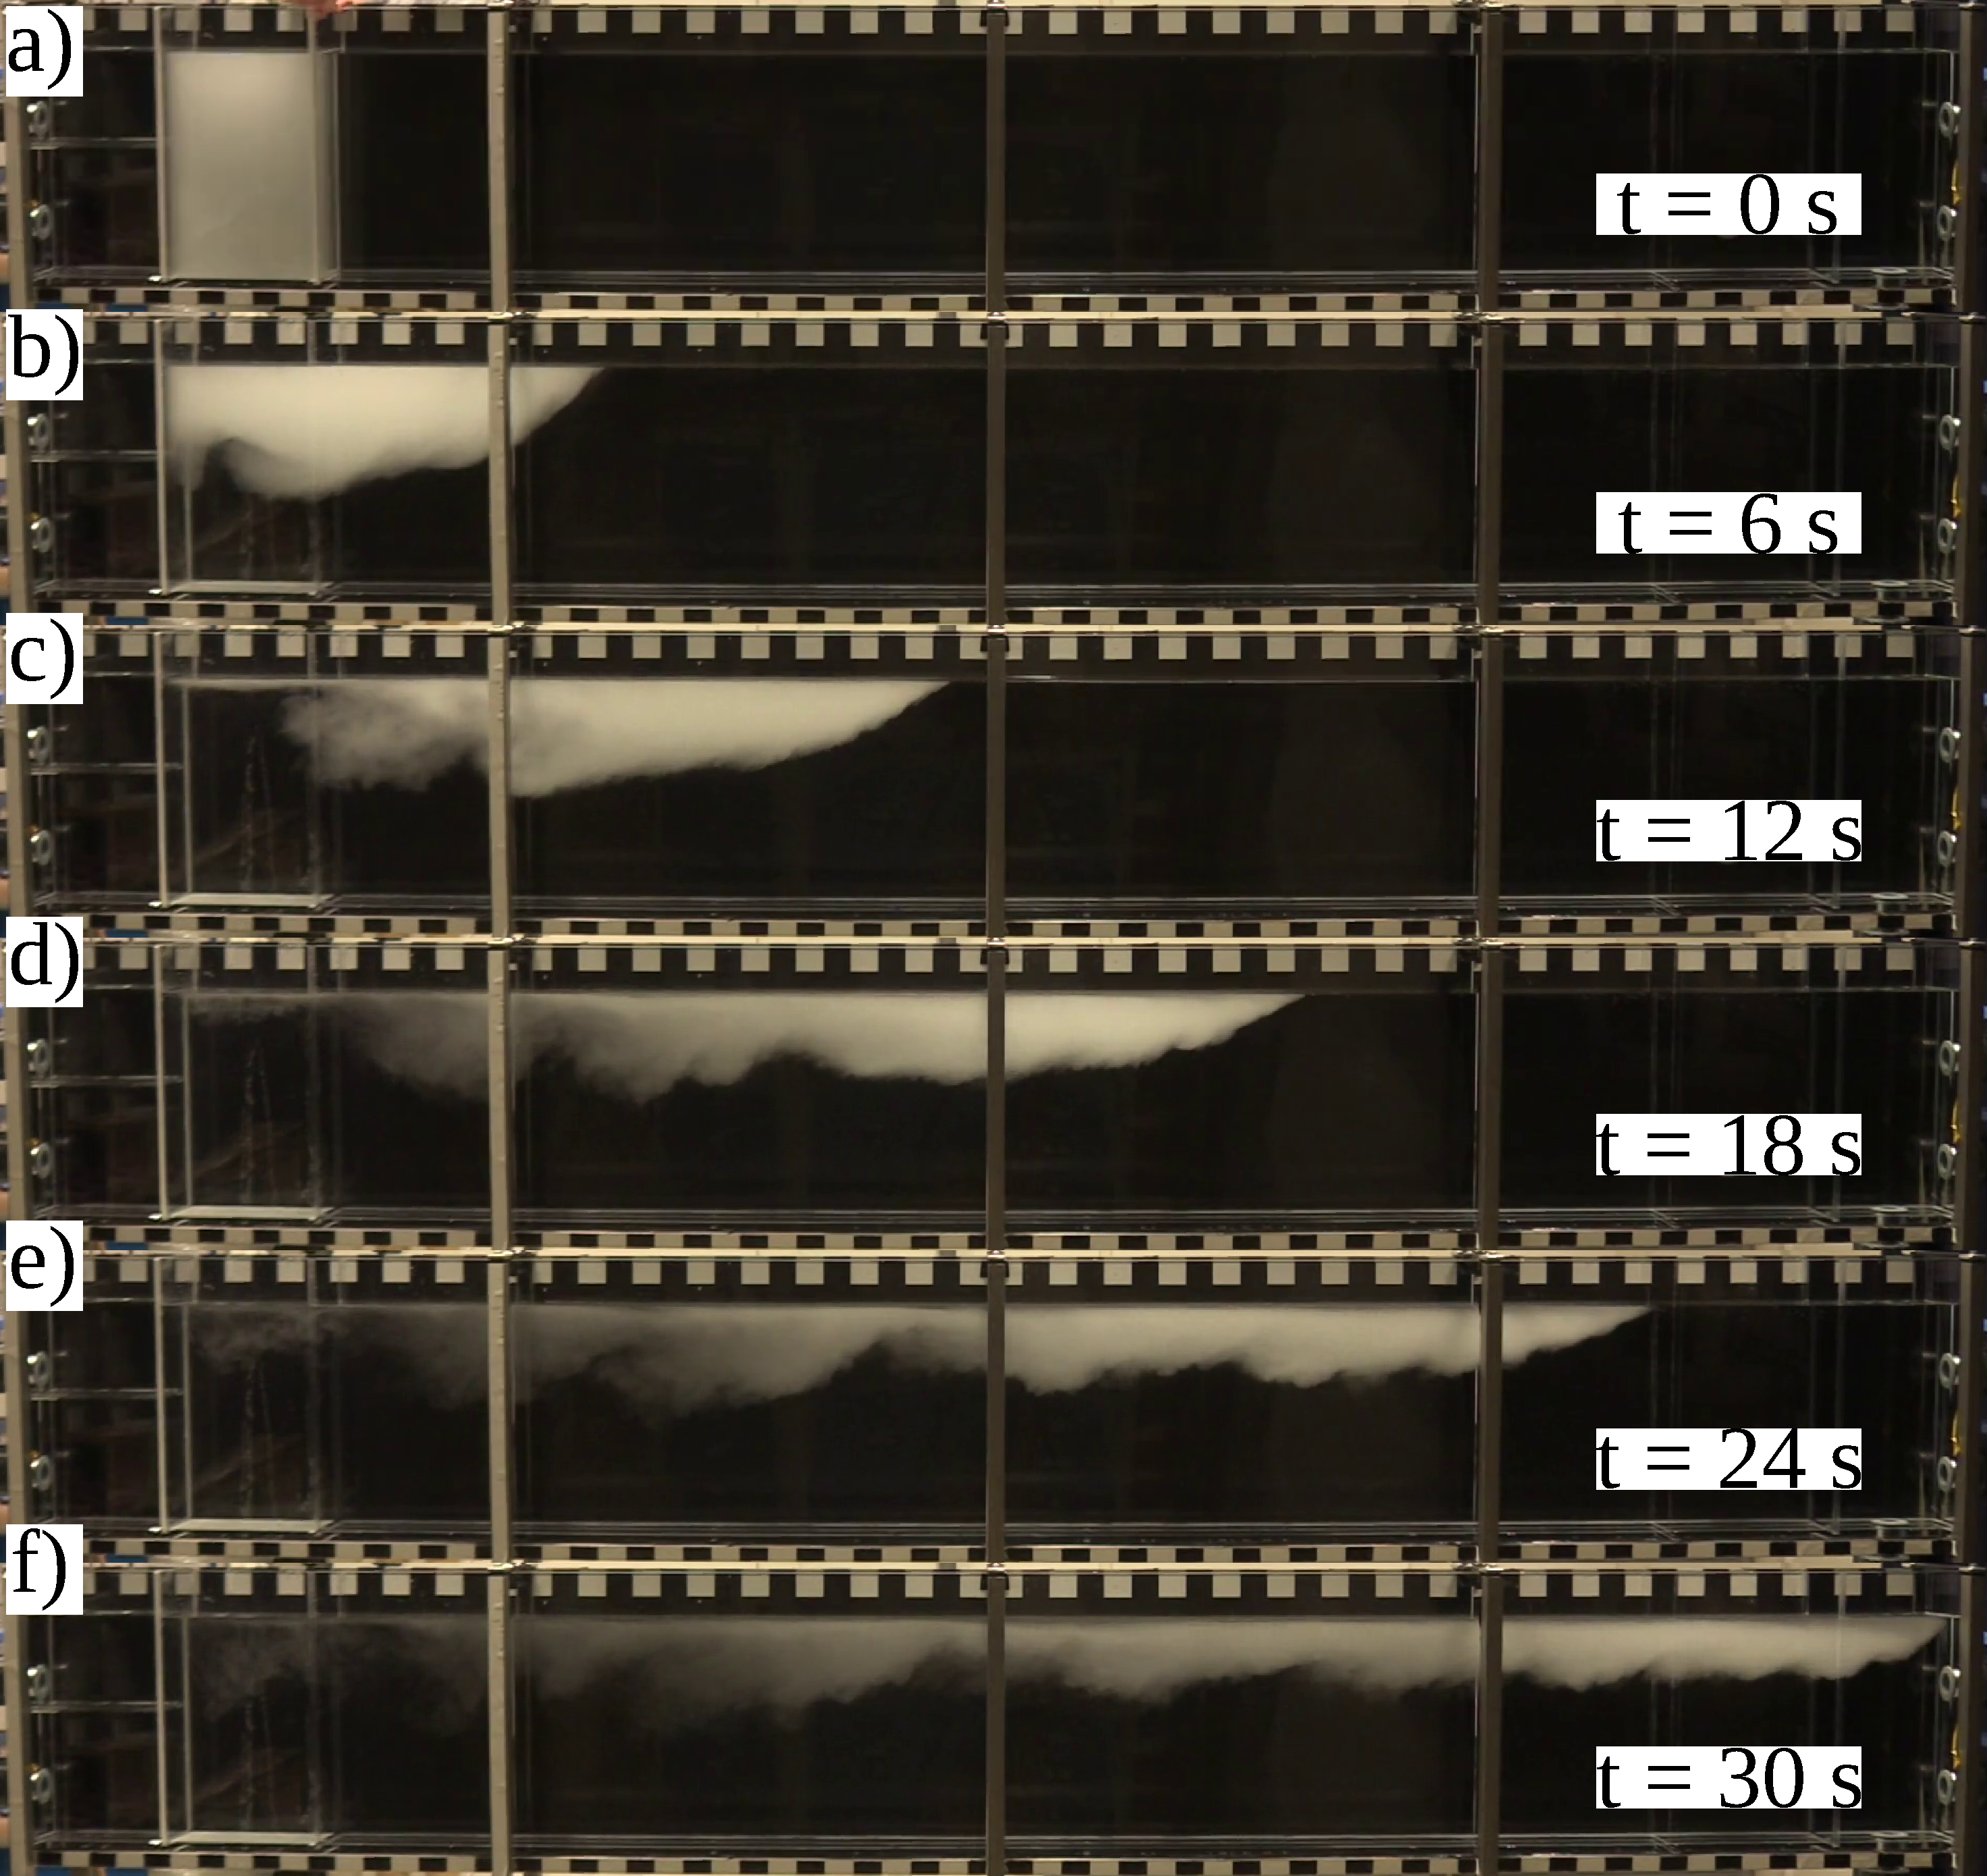
\includegraphics[width=0.9\textwidth]{GC42.pdf}}
  \caption{Sequence of images showing experiment GC42. }
  \label{fig:GC42}
\end{figure}

Figure~\ref{fig:GC48} shows the evolution of the current in experiment GC48.

\begin{figure}[ht!]
  \centerline{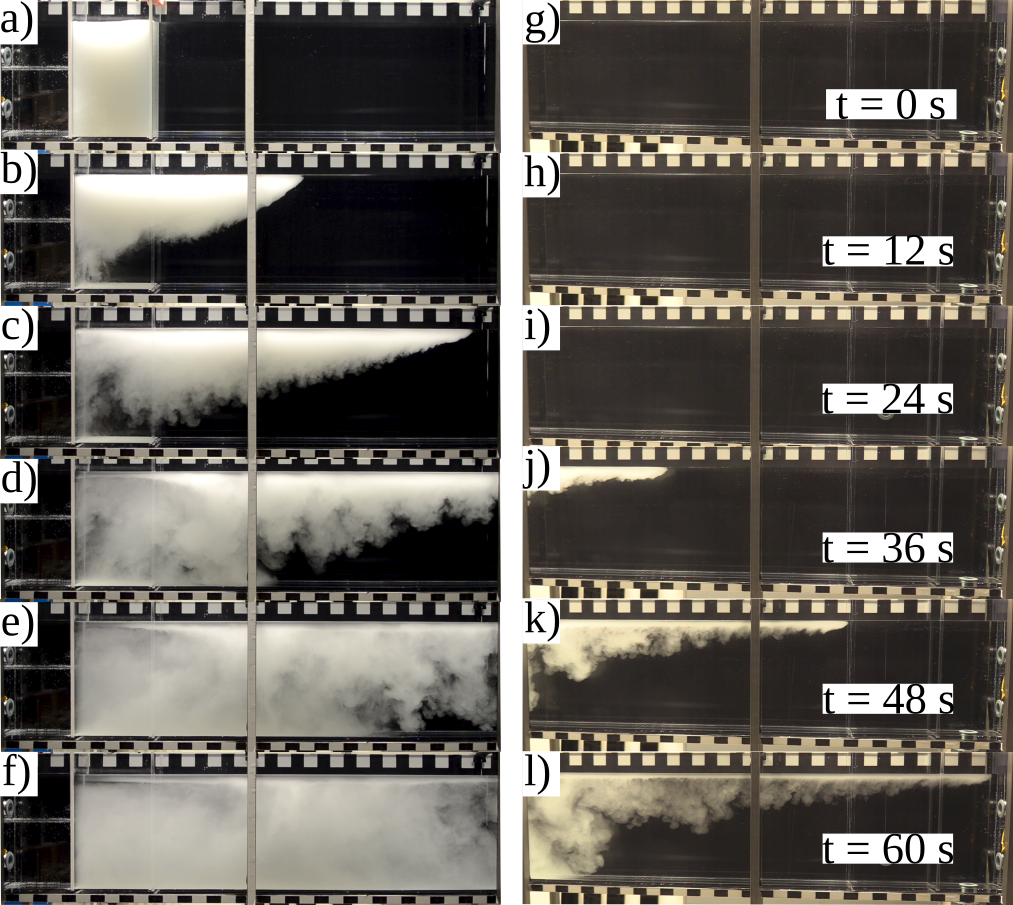
\includegraphics[width=0.9\textwidth]{GC48.pdf}}
  \caption{Sequence of images showing experiment GC48. a-f) show the left hand side of the tank whilst g-l) show the right hand side.}
  \label{fig:GC48}
\end{figure}

Figure~\ref{fig:GC45} shows the evolution of the current in experiment GC45.

\begin{figure}[ht!]
  \centerline{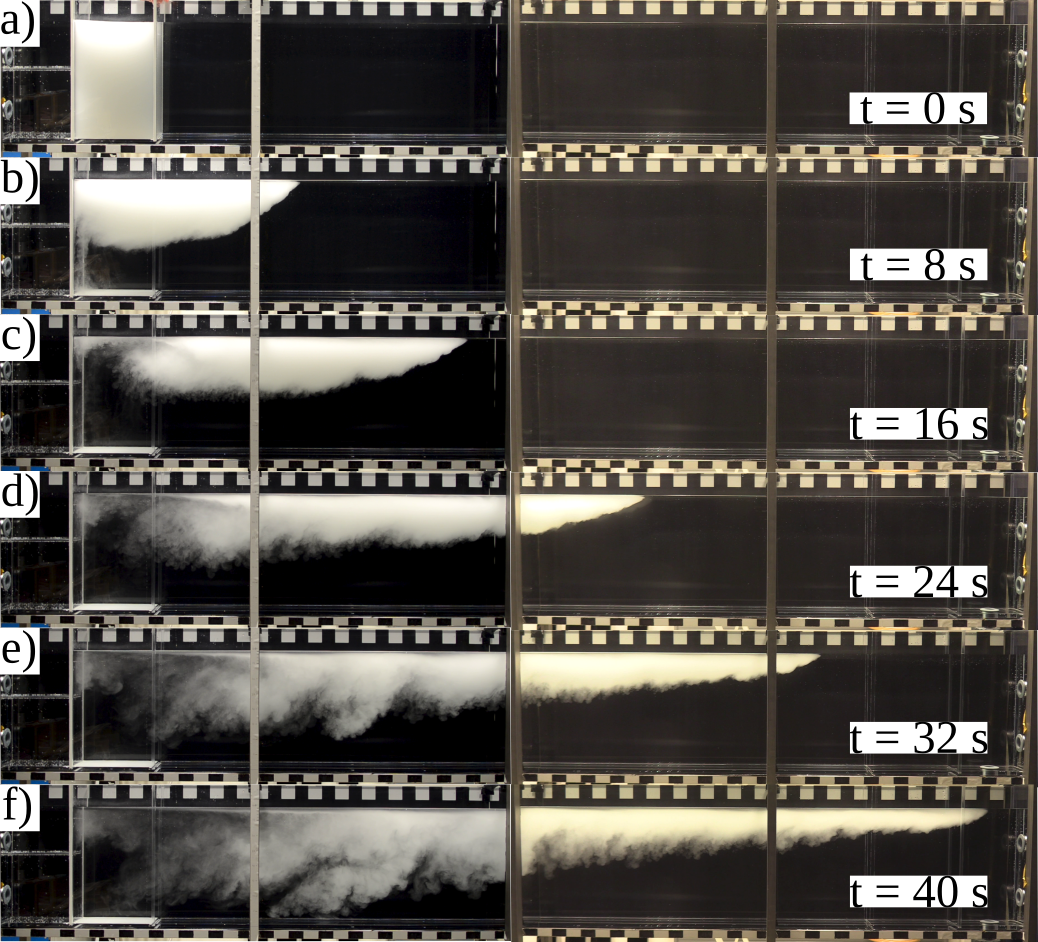
\includegraphics[width=0.9\textwidth]{GC45.pdf}}
  \caption{Sequence of images showing experiment GC45. a-f) show the left hand side of the tank whilst g-l) show the right hand side.}
  \label{fig:GC45}
\end{figure}

\section{Discussion}
\label{sec:dis}

\section{Conclusions}
\label{sec:conc}

\section*{Acknowledgements}
\label{sec:acknow}


%% The Appendices part is started with the command \appendix;
%% appendix sections are then done as normal sections
%% \appendix

%% \section{}
%% \label{}

%% If you have bibdatabase file and want bibtex to generate the
%% bibitems, please use
%%
%\bibliographystyle{elsarticle-harv}
%\bibliographystyle{elsarticle-num} 
\bibliographystyle{model2-names.bst}\biboptions{authoryear}
\bibliography{grav_current.bib}

%% else use the following coding to input the bibitems directly in the
%% TeX file.

%\begin{thebibliography}{00}

%% \bibitem[Author(year)]{label}
%% Text of bibliographic item

%\bibitem[ ()]{}

%\end{thebibliography}
\end{document}

\endinput
%%
%% End of file `elsarticle-template-harv.tex'.
